\documentclass{standalone}
\usepackage{tikz}
\begin{document}
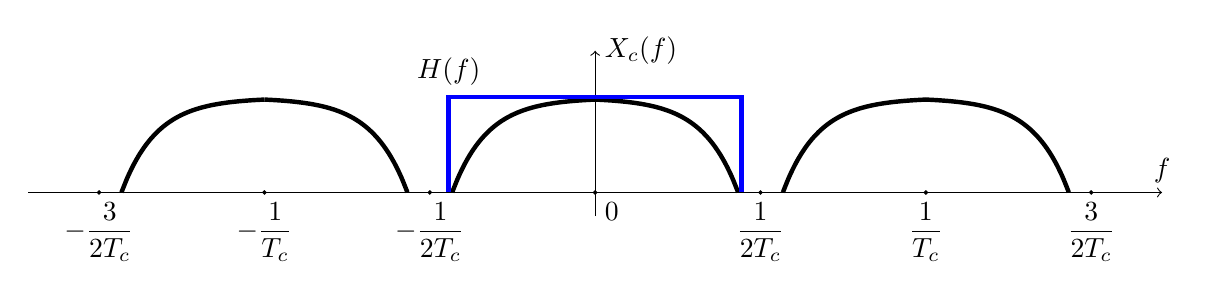
\begin{tikzpicture}[scale=1.2]
    \draw[->](-6,0)--(6,0)node[above]{$f$};
    \draw[->](0,-0.25)--(0,1.5)node[right]{$X_c(f)$};

    \draw[ultra thick]plot[smooth, domain=0:1.513](\x,{1-0.25*e^(2.7*(\x-1))});
    \draw[ultra thick]plot[smooth, domain=-1.513:0](\x,{1-0.25*e^(-2.7*(\x+1))});

    \draw[ultra thick]plot[smooth, domain=-3.5:-1.987](\x,{1-0.25*e^(2.7*(\x+2.5))});
    \draw[ultra thick]plot[smooth, domain=-5.013:-3.5](\x,{1-0.25*e^(-2.7*(\x+4.5))});

    \draw[ultra thick]plot[smooth, domain=3.5:5.013](\x,{1-0.25*e^(2.7*(\x-4.5))});
    \draw[ultra thick]plot[smooth, domain=1.987:3.5](\x,{1-0.25*e^(-2.7*(\x-2.5))});

    \draw[-,ultra thick, blue](1.55,0)--(1.55,1.01)--(-1.55,1.01)node[above, black]{$H(f)$}--(-1.55,0);

    \filldraw[black](1.75,0)node[below]{$\displaystyle\frac{1}{2T_c}$}circle(0.5pt);
    \filldraw[black](-1.75,0)node[below]{$\displaystyle-\frac{1}{2T_c}$}circle(0.5pt);
    \filldraw[black](3.5,0)node[below]{$\displaystyle\frac{1}{T_c}$}circle(0.5pt);
    \filldraw[black](-3.5,0)node[below]{$-\displaystyle\frac{1}{T_c}$}circle(0.5pt);
    \filldraw[black](5.25,0)node[below]{$\displaystyle\frac{3}{2T_c}$}circle(0.5pt);
    \filldraw[black](-5.25,0)node[below]{$\displaystyle-\frac{3}{2T_c}$}circle(0.5pt);
    \filldraw[black](0,0)node[below right]{$0$}circle(0.5pt);
\end{tikzpicture}
\end{document}